\ifx\allfiles\undefined
\documentclass{XDBAthesis}
\def\pictures{}
\numberwithin{algorithm}{chapter}
\floatname{algorithm}{算法}
\renewcommand{\algorithmicrequire}{\textbf{输入:}}
\renewcommand{\algorithmicensure}{\textbf{输出:}}
\begin{document}
\else
\fi
\chapter{基于二次哈希开链法的图精确搜索}
\label{chap:graphgrep}
由于传统算法在利用哈希表存储索引中多采用简单哈希,容易产生冲突问题,导致构建索引效率较低。本章在路径索引的基础上,探究了不同哈希方法对算法速度的影响,并提出一种基于二次哈希开链法的精确搜索算法,来减少图搜索中的过滤阶段的耗时,以提高搜索速度。本章将先介绍下现有的哈希算法,然后详细介绍基于二次哈希开链法搜索的搜索方法包括作为此算法验证方法用的子图同构算法\emph{ULLMANN}\cite{ullmann}。最后是实验结果与分析。

\section{常用哈希方法}
本节将介绍三种常用的解决哈希冲突的方法,开放定址法,开链法,再哈希法。

\subsection{开放定址法}
开放定址法\cite{datastruct}是一种常用的处理冲突方法,公式如\eqref{eq:open}所示
\begin{equation}
    H_i =(H(key)+d_i )MOD\ m\ \  \ i=1,2,...,k(k\leq m-1)
    \label{eq:open}
\end{equation}

其中,$H(key)$为哈希函数;$m$为哈希表表长,$d_i $为增量序列,可有以下三种取法:
\begin{enumerate}
    \item $d_i =1,2,3,...,m-1$,称线性探测再散列;
    \item $d_i =1^2 ,-1^2 ,2^2 ,-2^2 ,3^2 ,...,\pm k^2 ,(k\leq m/2 ) $,称为二次探测再散列;
    \item $d_i =$伪随机数序列,称为伪随机探测再散列。
\end{enumerate}
\subsection{开链法}
开链法又称链地址法\cite{datastruct},是将所有关键字为同义词的记录存储在同一线性链表中。
\subsection{再哈希法}
\begin{equation}
    H_i =RH_i (key)\ i=1,2,...,k
    \label{eq:twice}
\end{equation}
再哈希法\cite{datastruct}如公式\eqref{eq:twice}所示,$RH_i $均是不同的哈希函数,即在同义词产生地址冲突时计算另一个哈希函数地址,直到冲突不再发生。
\section{基于二次哈希开链法的搜索算法}
本方法同\emph{GraphGrep}算法\cite{graphgrep},都是基于路径的精确子图搜索算法。算法基本流程如下:(1)遍历图数据库中图的路径,(2)利用双哈希构建索引,(3)遍历查询图路径,(4)利用基本索引特征先验剪枝,(5)路径合成进一步筛选候选集,(6)子图同构确定最终结果。下面我们将分小节详细说明这些步骤。
\subsection{数据库路径遍历}
首先,对于每个数据库我们设定一个路径长度的上限$l_p $,$l_p $越大意味着可记录的路径越长,索引集合也会相应增加。随后对于数据库中的每幅图,我们用深度优先搜索遍历每个节点,遍历最大深度为$l_p $,并记录遍历过程中经过的每一条路径,存成一个列表,用于下一步构建索引。
\subsection{二次哈希开链法索引构建}
双哈希是再哈希的一种,其利用两个哈希函数来构造哈希探测序列,大大降低了地址冲突概率。但是传统上,双哈希方法实质上也是开放定址法的一种,也就是如果所需节点数目大于$Mod$时,将完全无法表示。这完全不符合图数据库实际情况,因为作为一个通用算法,我们无法预先确定数据库中最大图的节点数。因此,本文将双哈希和开链法相结合提出了一个变形的双哈希算法,即\emph{二次哈希开链法}来进行哈希定址。

二次哈希开链法就是只进行一次双哈希,然后再有冲突就利用开链法解决。双哈希函数公式如\eqref{eq:hash_e}。
\begin{equation}
    h(key)=(h_1 (key)+ h_2 (key))\%Mod
    \label{eq:hash_e}
\end{equation}

其中$h_1 ,h_2 $为两个不同的哈希函数,$Mod$为哈希函数取模值,一般为一个小于但最接近存储空间大小的素数。当$h_1 (key)$发生冲突时,再用$h_2 (key)$的值作为偏移量来进行探测。如果再有冲突则进行开链法,存成链表。

根据二次哈希开链法的特点,本文设计了一种将路径字符串映射到哈希表的算法,如算法\ref{algo:hashcode}所示。而访问时函数则不需重新设计,直接用开链法原有函数即可。

\begin{algorithm}
\caption{二次哈希编码}
\label{algo:hashcode}
\begin{algorithmic}[1]
    \Require 路径字符串 $path\_string$
    \Ensure 哈希编码 $code$
    \Function {hash}{$path\_string$}
        \State $code \gets h_1 (key)\%Mod$
        \If {$code$有冲突}
            \State $code \gets (code+h_2 (key))\%Mod$
        \EndIf
        \State \Return{$code$}
    \EndFunction     
\end{algorithmic}
\end{algorithm}

在二次哈希开链法中哈希函数可以自选,不过我们推荐选取算法\ref{algo:hashfunction}中的两个函数作为$h_1 ,h_2 $,经过实验这两个函数对于字符串哈希这两个效果最好。

\begin{algorithm}
\caption{哈希函数}
\label{algo:hashfunction}
\begin{algorithmic}[1]
    \Require 字符串 $String$
    \Ensure 哈希编码 $code$
    \Function {$h_1 $}{$String$}\Comment{BKDRHash}
        \State $char \gets (string.first)$
        \State $code \gets 0$
        \While {$char \neq 0 $}
            \State $code \gets code<<6+char$
            \State $char \gets (char.next)$
        \EndWhile
        \State \Return{$(code\&0\times 7FFFFFFF)\%Mod$}
    \EndFunction
    \Function {$h_2 $}{$String$}\Comment{APHash}
        \State $char \gets (string.first)$
        \State $code \gets 0$
        \State $i \gets 0 $
        \While {$char \neq 0 $}
            \If{$i$为偶数}
                \State $code \gets (code\oplus ((code<<7)\oplus char\oplus (code>>3))$
            \Else
                \State $code \gets (code\oplus (\sim ((code<<11)\oplus char\oplus (code>>5)))  $
            \EndIf
            \State $char \gets (char.next)$
        \EndWhile
        \State \Return{$(code\&0\times 7FFFFFFF)\%Mod$}
    \EndFunction          
\end{algorithmic}
\end{algorithm}

\emph{BKDRHash}运算简单,速度快,所以作为第一次哈希函数。\emph{APHash}不易冲突,所以作为第二次。

通过哈希存储,我们可以很便捷得获得各图包含的路径关系表,我们将其存到文件中作为索引,分离查询与建库,进行离线查询加速查询速度。

\subsection{查询图路径遍历}
我们对查询图也像数据库中的图一样进行拆分,以$l_p $为路径最大长度遍历出所有路径。然后同样存成一个哈希表,记录着每一条路径出现了几次。为进一步搜索做准备。不过和数据库路径遍历有所不同的是,查询图的遍历过程中需要记录不同路径中相同的节点,这个可以通过在路径中添加特定标签实现。
\subsection{先验剪枝}
    在介绍本算法的先验剪枝步骤之前,我们先介绍一下\emph{包含逻辑规则(inclusion logic)}。
    \begin{defn}[包含逻辑]\cite{inclusionlogic}
        对于给定的标号图$g_1 ,g_2 $,和$g_1 $的一个子图$g'$,若$g_1 $是$g_2 $的子图,则$g'$必定是$g_2 $的子图$(g_1 \subseteq g_2 ) \Rightarrow (g' \subseteq g_2  )$。反之,若$g'$不是$g_2 $的子图,则$g_1 $也不可能是$g_2 $的子图$(g' \not\subset g_2  )\Rightarrow (g_1 \not\subset g_2 )$    
    \end{defn}
    从包含逻辑规则中,我们可以得知如果查询图$g_1 $中的子图$g'$不是数据图$g_2 $的子图,那么$g_2 $就不可能是$g_1 $的超图,因此可以放心得把$g_2 $从候选集中删去。这就大大加速了“过滤-验证”框架中过滤阶段的过滤速度。
    
    在本算法中,我们从三个方面进行了先验剪枝来缩小索引集个数。三个方面分别是(i)节点,(ii)边,(iii)路径。如果查询图中的某个节点个数大于数据图中的,那么数据图自然不会包含查询图。如果查询图中有数据图中没有的边,那么自然这幅数据图也不合要求。如果查询图中某条路径的个数大于数据图,那么因为包含逻辑规则,这幅数据图也当从候选集中删去。
    
    经过这三步筛选过程,候选集将会大大减少,降低了后文所述路径合成和子图同构所需时间。
\subsection{路径合成}
当完成先验剪枝后,候选集已经相对较小,但是并没有达到最好的情况。我们可以通过路径合成确定其中很多的合理性。路径合成的复杂度远远小于子图同构,因此最后对候选集做一次路径合成可以大大降低最终复杂度。
路径合成,顾名思义就是将多条路径进行合成,具体而言就是将多个有着公共节点的路径合成到一起,通过判定其是不是相同节点来筛选候选集。我们采用的是遍历的方法,只进行两两合成,然后逐一比对。如例\ref{exmp:pathcombine}所示。
\begin{exmp}
    假设有路径$\bar{A}B\underbar{C}\bar{A} $和$\underbar{C}B$,其中有相同标记的节点均为同一节点,即在本例中两个$A$是同一节点和两个$C$也是同一节点。
    \label{exmp:pathcombine}
    \begin{enumerate}
        \item 现在假设数据库中有四幅图,其路径信息如下所示,数字代表节点标识:
        $$
        \begin{aligned}
            g_1 &:ABCA={(1,0,3,1)}\ CB={(3,2)}\\
            g_2 &:ABCA={(1,2,3,1)}\ CB={(3,2)}\\
            g_3 &:ABCA={(1,0,3,4)}\ CB={(3,2)}\\
            g_4 &:ABCA={(1,0,4,1)}\ CB={(3,2)}\\
        \end{aligned}
        $$
        \item 在路径合成前,我们就可以利用节点信息删去$g_3$,因为$g_3$的$ABCA$中两个$A$一个是1,一个是4,并非同一节点。
        \item 我们将ABCA和CB合成,我们知道其中两个$A$是统一节点,两个$C$是同一节点,而两个$B$不是。我们得到合成结果:
        $$
        \begin{aligned}
            g_1 &:ABCACB={(1,0,3,1),(3,2)}\\
            g_2 &:ABCACB={(1,2,3,1),(3,2)}\\
            g_4 &:ABCACB={(1,0,4,1),(3,2)}\\
        \end{aligned}
        $$
        \item  显然,$g_2$不满足条件,因为它的两个$B$也是一个节点,$g_4$也不满足,因为其两个$C$不是同一节点。所以筛选集中只剩下$g_1$。
    \end{enumerate}    
\end{exmp}
可见,通过路径合成,我们大大缩小了候选集,降低了下一步子图同构所需的计算量,加速了整个算法。

\subsection{子图同构}
子图同构作为算法最后的验证部分,承担着对于整个算法正确性把关的责任,也同样是个需要消耗大量运算量的部分。由于子图同构是个$NP-hard$问题,所以目前仍没有一种快速的解法。我们选用经典算法\emph{ULLMANN}算法\cite{ullmann}来解决这个问题。下面我们将大致介绍下UllMANN算法。

ULLMANN算法是Ullmann教授1976年提出的一种经典图同构算法,其本质是基于一个深度优先搜索树。其算法流程如图\ref{fg:ullmanchart}所示。首先,根据查询图节点的出入度从数据图中找出候选集。随后,再根据每个节点的邻接节点对候选集进行筛选。最后,通过深度优先搜索,一一遍历配对,寻找匹配点。例\ref{exmp:ullmann}就是一个子图同构的完整过程。
\todo{补充Ullmann图和例子}
\begin{figure}
    \caption{Ullmann算法流程图}
    \label{fg:ullmanchart}
\end{figure}
\begin{exmp}
    \label{exmp:ullmann}    
\end{exmp}


\section{实验结果与分析}
\subsection{实验环境}
本文提出算法的实验环境为CPU Intel Core i7,主频为1.7 GHz,内存为8 GB 1600 MHz DDR3,硬盘为128GB SSD,操作系统为Mac OS X Yosemite 10.10.3;所有算法均用C语言在clang 600.0.56环境编译完成。
\subsection{实验数据分析}
实验数据全采用真实数据,为DTP提供的AIDS数据集。可从以下网址得到:\url{https://wiki.nci.nih.gov/display/NCIDTPdata/AIDS+Antiviral+Screen+Data}。我们从其数据库中随机抽取了1000,2000,4000,8000,16000个图作为我们的查询集合。数据集平均每幅图有41条节点,48条边。所有实验运行10次取平均值。

实验结果如图\ref{fg:THCBuild},\ref{fg:THCRun}所示,THC为Twice Hash Chain(二次哈希开链法)的缩写。我们测试了不同最大长度$l_p $下两个算法的表现。
\begin{figure}[htb]
    \centering
    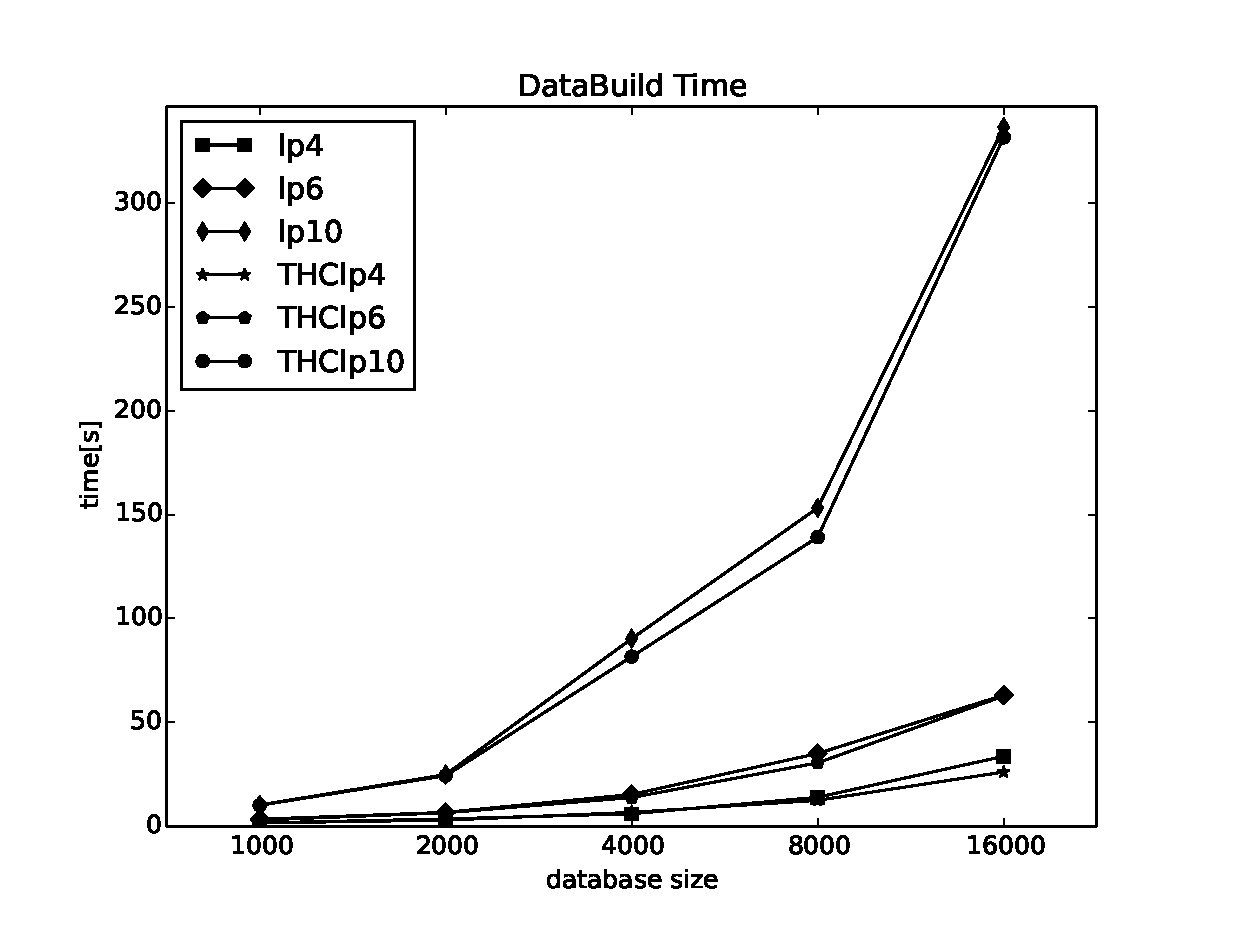
\includegraphics[width=0.5\textwidth]{../figures/THC/BuildCompare_4_6_10}%
    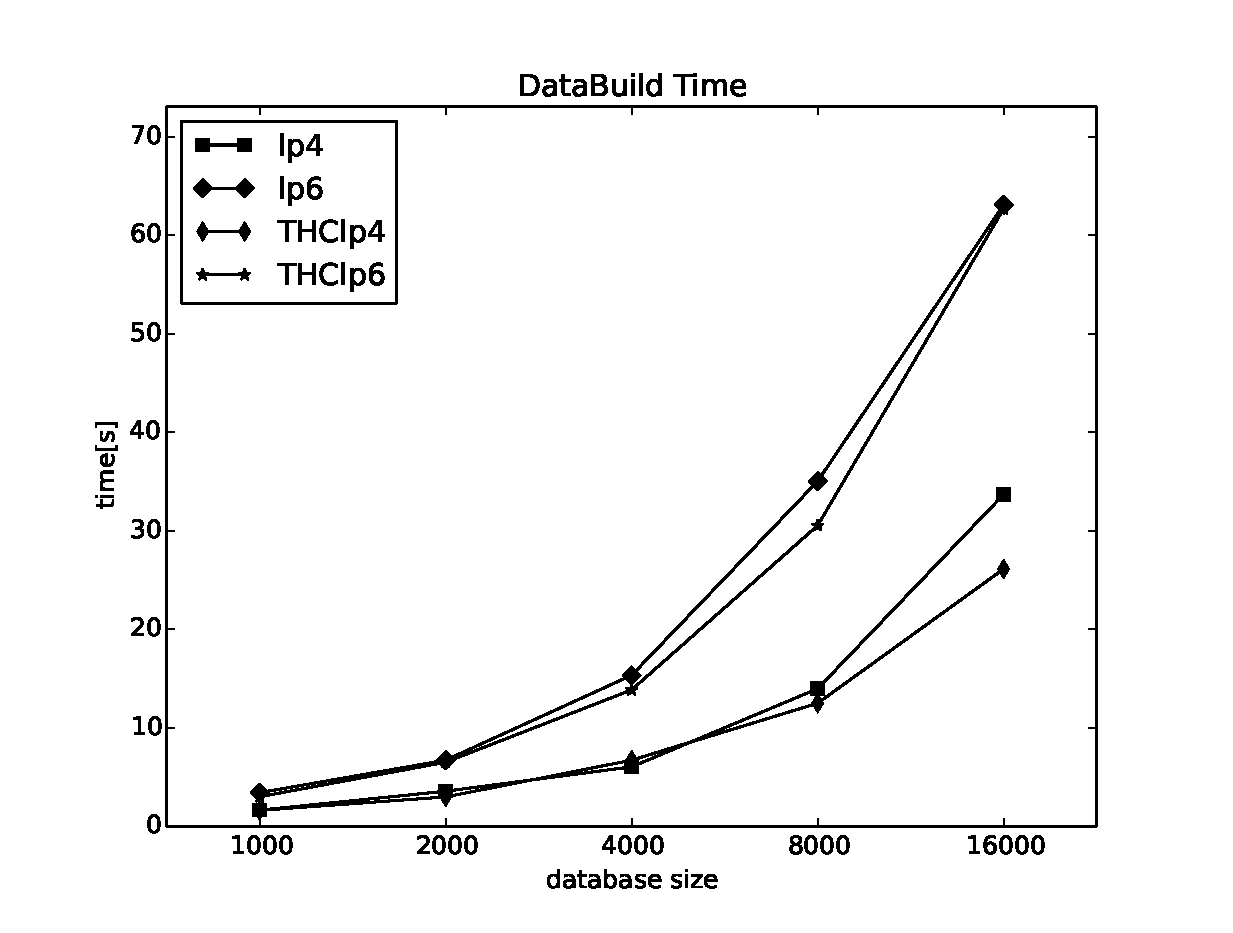
\includegraphics[width=0.5\textwidth]{../figures/THC/BuildCompare_4_6}
    \caption{建库时间比较}
    \label{fg:THCBuild}
\end{figure}
\begin{figure}[htb]
    \centering
    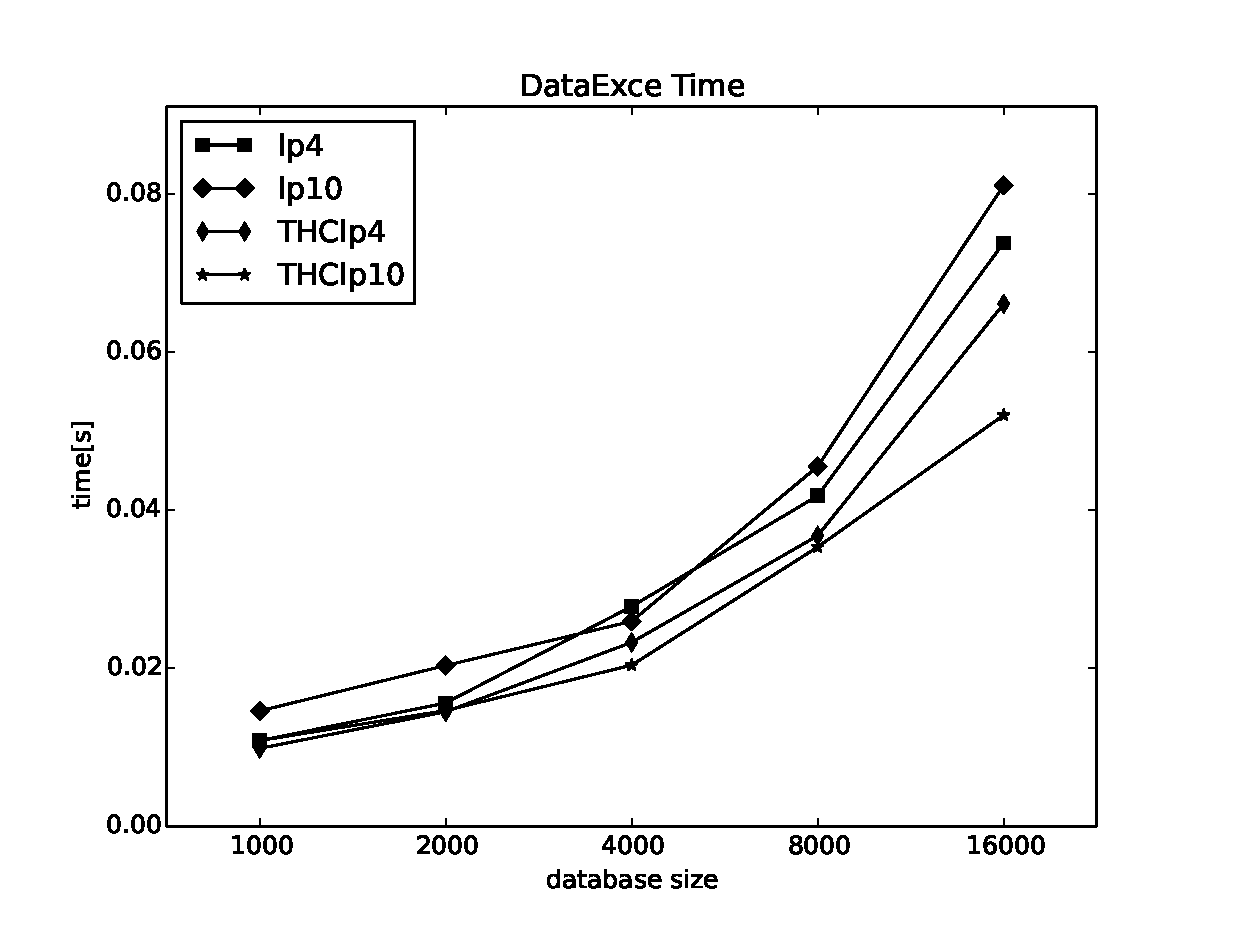
\includegraphics[width=\textwidth]{../figures/THC/ExceCompare_4_10}
    \caption{运行时间比较}
    \label{fg:THCRun}
\end{figure}

由图可知,二次哈希开链的确有效减少了冲突,提高了建库速度与查询速度。

\ifx\allfiles\undefined
\bibliographystyle{unsrt}
\bibliography{main}
\end{document}
\fi